% =========================================================================== %
% TeX input file: "Create a new project"
%
% WARNING: this tex file does not compile standalone, it needs to be embedded
% in a master tex document (e.g. Introduction.tex)
% =========================================================================== %

Start your Eclipse IDE and select an empty directory for your workspace. 
This workspace directory will then hold all the project code for the ''Hello World'' application. 
Once the Eclipse IDE is running it will show the Scout perspective with the ''Scout Explorer'' view and an empty ''Scout Object Properties'' view.
To create a new Scout project select the \contextmenu{New Scout Project...} as shown in \figref{sdk_create_new_scout_project}.

\begin{figure}
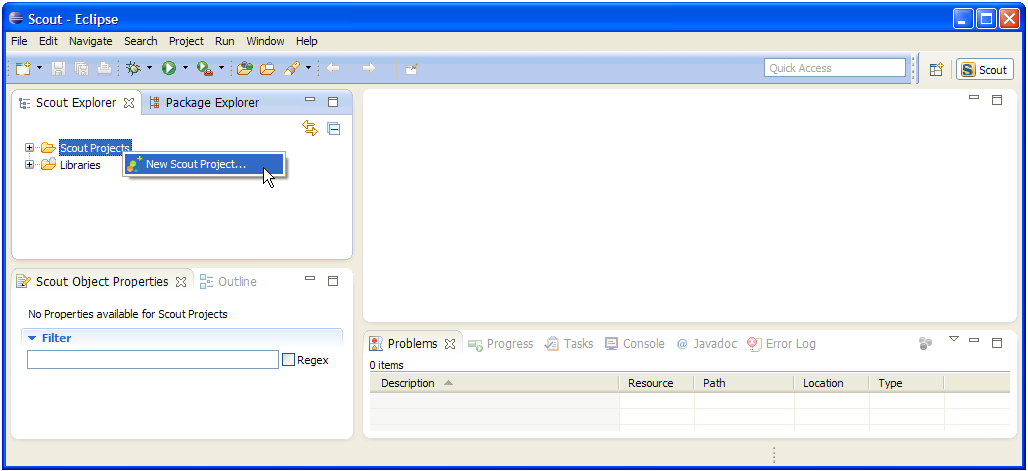
\includegraphics[width=15cm]{sdk_create_new_scout_project.png}
\caption{Create a new Scout project using the Scout SDK perspective.}
\figlabel{sdk_create_new_scout_project}
\end{figure}

In the \wizard{New Scout Project} enter a name for your Scout project. 
As we are creating a ''Hello World'' application, use \java{org.eclipsescout.helloworld} for the \field{Project Name} according to \figref{sdk_new_project_wizard}.
Then, click the \button{Finish} to let the Scout SDK create the initial project code for you.

\begin{figure}
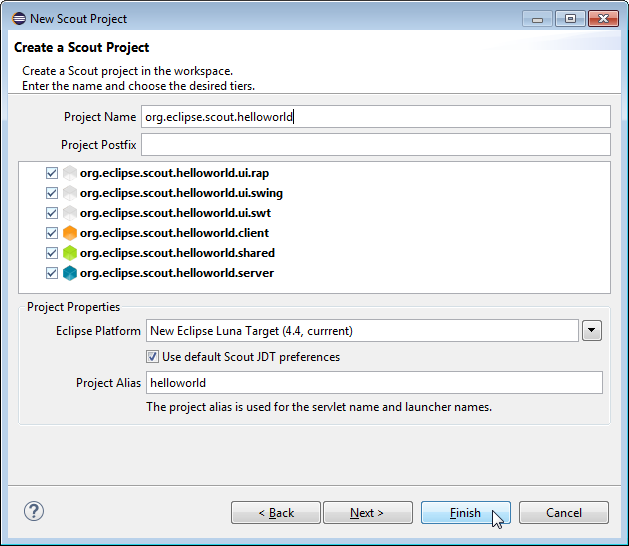
\includegraphics[width=6cm]{sdk_new_project_2.png}
\caption{The new Scout project wizard.}
\index{SDK Wizard!New Scout Project}
\figlabel{sdk_new_project_wizard}
\end{figure}

Once the initial project code is built, the Scout SDK displays the application model in the \textit{Scout Explorer} as shown in \figref{sdk_initial_helloworld_project}.
This model is visually presented as a tree structure covering both the client and the server part of the application.
The Scout Explorer view on the left hand side displays the top level elements of the complete Scout application.
Under the orange node the Scout client components are listed. 
Components that are needed in both the Scout client and the Scout server are collected under the green node.
And the Scout server components are listed below the blue node in the Scout Explorer view.

\begin{figure}
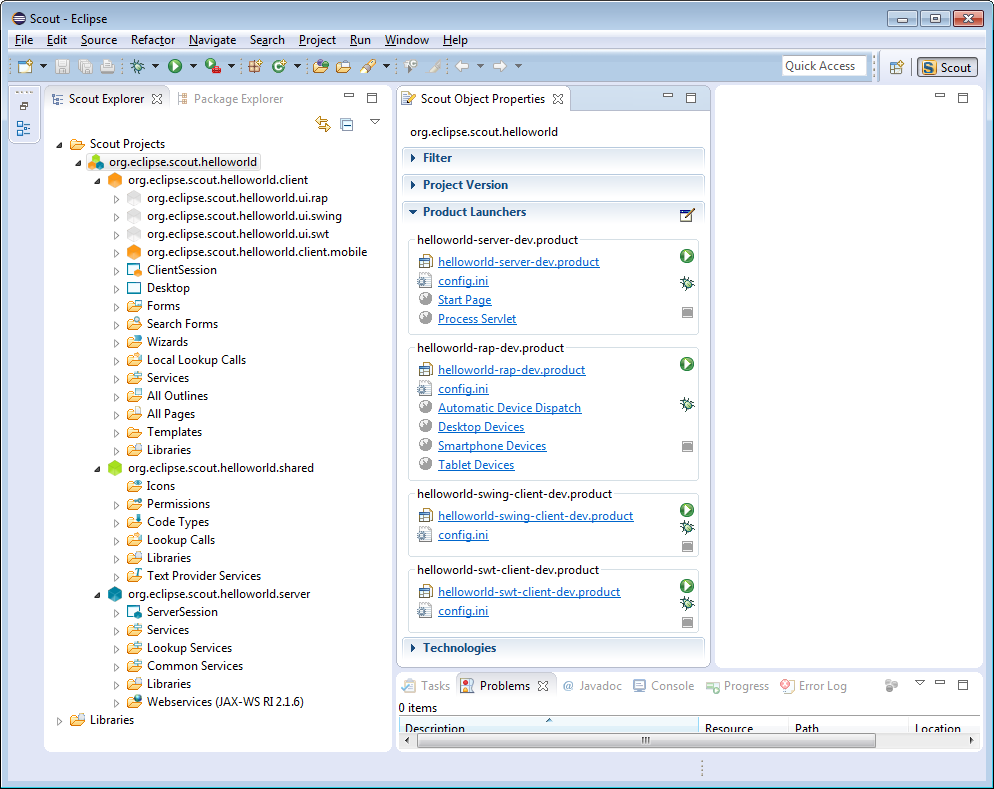
\includegraphics[width=15cm]{sdk_initial_helloworld_project.png}
\caption{The Scout SDK showing the tree representation of our ''Hello World'' application in the Scout Explorer.
The Scout Object Properties contain the product launchers for the server and the available clients.}
\figlabel{sdk_initial_helloworld_project}
\end{figure}

% =========================================================================== %
% EOF TeX input file
% =========================================================================== %
